\documentclass[a4paper, onecolumn]{article}
\usepackage[english]{babel}
\usepackage{caption}
\usepackage{graphicx}
\usepackage{amsmath}
% Configure bibtext
\usepackage{cite}
\setlength{\parindent}{0pt}

\author{Josué Villasante}
\title{Amplitude damping channel}

\begin{document}
	\maketitle

	\section{One qubit}
		The amplitude damping channel (ADC) is defined by the map \cite{yugra_constraints_2022}
		$$
		\begin{gathered}
			|00\rangle \rightarrow|00\rangle \\
			|10\rangle \rightarrow \sqrt{1-p}|10\rangle+\sqrt{p}|01\rangle
		\end{gathered}
		$$
		applied on two qubits, the second one being the environment. If we we consider a state of one qubit given by
		\begin{equation}
			|\psi\rangle = \cos\theta|0\rangle + \sin\theta|1\rangle
		\label{q0_ini}
		\end{equation}
		then to apply the ADC we consider a state $|\psi0\rangle$, where the second qubit belongs to the environment. The final state of the whole system would be
		$$
		|\phi\rangle = \cos\theta|00\rangle + 
					   \sin\theta(\sqrt{1-p}|10\rangle + \sqrt{p}|01\rangle)
		$$

		In general a circuit like \ref{adc_1q} produces the ADC for any initial state of the qubit 0.

		\begin{center}
			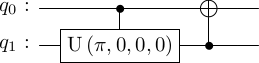
\includegraphics[width=100pt]{img/adc_1q.png}
			\captionof{figure}{ADC for one qubit. \cite{nielsen_quantum_2010}}
			\label{adc_1q}
		\end{center}

		Here the U gate is defined \cite{Qiskit} by

		$$
		U(\theta, \phi, \lambda)=\left(\begin{array}{cc}
		\cos \left(\frac{\theta}{2}\right) & -e^{i \lambda} \sin \left(\frac{\theta}{2}\right) \\
		e^{i \phi} \sin \left(\frac{\theta}{2}\right) & e^{i(\phi+\lambda)} \cos \left(\frac{\theta}{2}\right)
		\end{array}\right)
		$$

		By using only the first parameter\footnote{The U gate on figure \ref{adc_1q} shows a value of $\pi$ but, in general, it may take any value. For all circuits in this papers this holds.} of the U gate we are left with a rotation matrix. Given that the qubit 0 may be initialized as equation \ref{q0_ini}, applying the circuit \ref{adc_1q} we are left with

		$$
		|\phi\rangle = \cos\theta|00\rangle + 
					   \sin\theta[\cos(\theta/2)|10\rangle + \sin(\theta/2)|01\rangle]
		$$
		
		where we must solve $\sin(\frac{\theta}{2}) = \sqrt{p}$ to apply a given value of $p$.

	\section{Two qubit}
		We may then consider a pure initial state of 2 qubits
		$$
		|\psi_i\rangle=\cos(\theta)|01\rangle + \sin(\theta)|10\rangle
		$$
		where the first qubit on the bracket corresponds to qubit 0 and the second to qubit 1. None belong to the environment yet. Then we consider the evolution of two qubits under a ADC, each with its environment qubit, $|\psi00\rangle$. We get
		$$
		|\phi_f\rangle=\cos \theta[\sqrt{1-p}|0100\rangle+\sqrt{p}|0001\rangle]+
		\sin \theta[\sqrt{1-p}|1000\rangle+\sqrt{p} |0010\rangle]
		$$
		To build a quantum circuit that outputs this state, we first, using qubit 0 and 1, build the state $|\psi_i\rangle$, and then using two more qubits apply a ADC to qubit 0 and 1. This way the environment of qubit 0 is qubit 2 and of qubit 1 is qubit 3. The first U gate prepares the initial state and the two remaining U gates, along with the CNOT gates, perform the ADC. Of the U gates only the first parameter is necessary.

		\begin{center}
			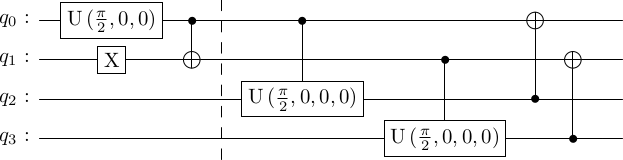
\includegraphics[width=300pt]{img/adc_2q_v0.png}
			\captionof{figure}{ADC for two qubit using two ancillas.}
			\label{adc_2q_v0}
		\end{center}

		Using this circuit we seek to show how a change in $p$ evolves a pure state to a mixed one. Using Qiskit quantum computer simulator we ran the circuit \ref{adc_2q_v0} with $\theta = \pi / 4$, performed a tomography on qubits 0 and 1, and obtained the following density matrices for different values of $p$.

		\begin{center}
			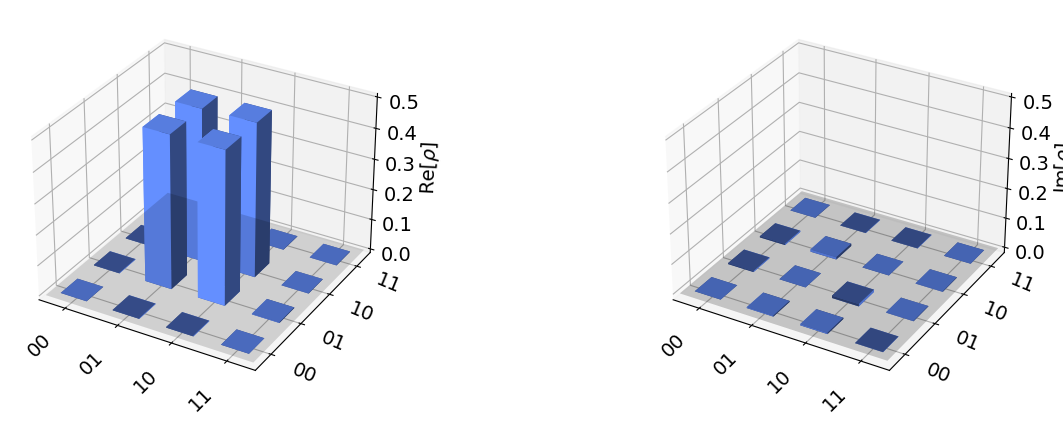
\includegraphics[width=300pt]{img/dm_p0_v0.png}
			\captionof{figure}{Final state for $p=0$.}
			\label{dm_p0}
		\end{center}

		\begin{center}
			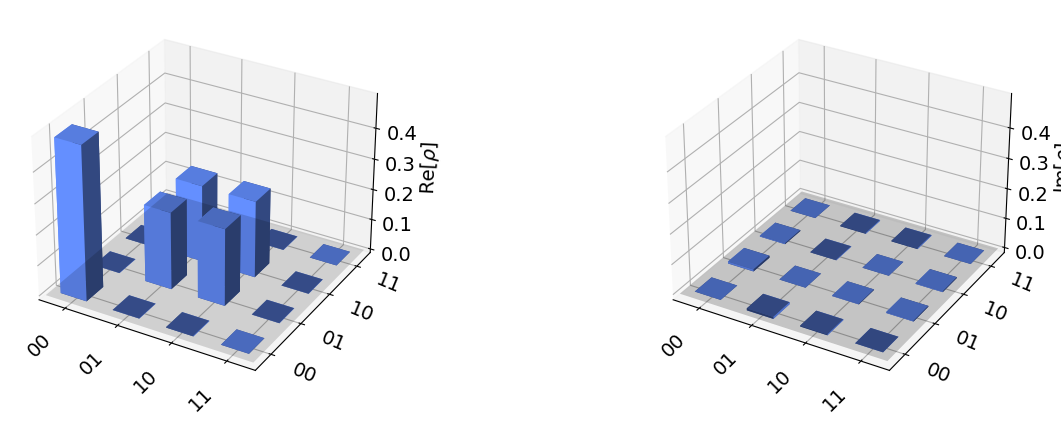
\includegraphics[width=300pt]{img/dm_p0.5_v0.png}
			\captionof{figure}{Final state for $p=0.5$.}
			\label{dm_p0.5}
		\end{center}

		\begin{center}
			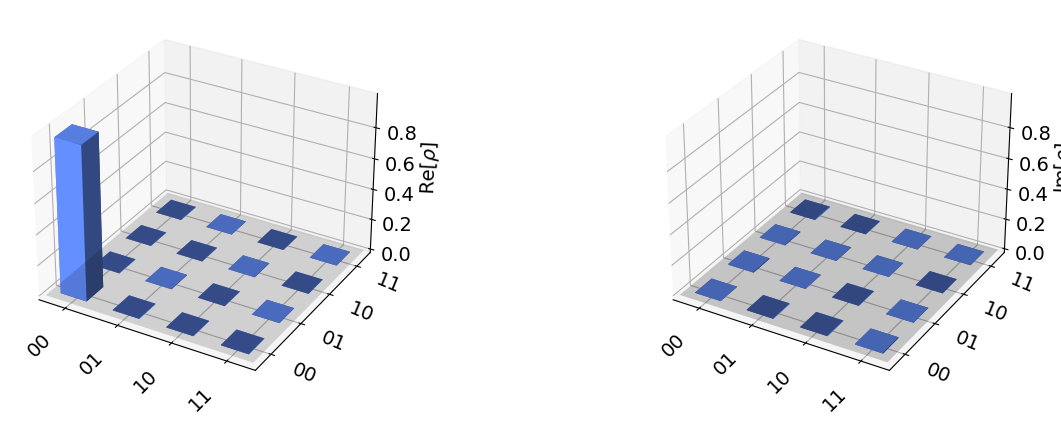
\includegraphics[width=300pt]{img/dm_p1_v0.png}
			\captionof{figure}{Final state for $p=1$.}
			\label{dm_p1}
		\end{center}

		We may also show that the relationship \cite{yugra_constraints_2022}
		\begin{equation}	
		\begin{aligned}
		& C_{01}^2+\left(P_0 \pm p\right)^2=(1-p)^2 \\
		& C_{01}^2+\left(P_1 \pm p\right)^2=(1-p)^2
		\end{aligned}
		\label{cp_relation}
		\end{equation}
		also holds.

		\begin{center}
			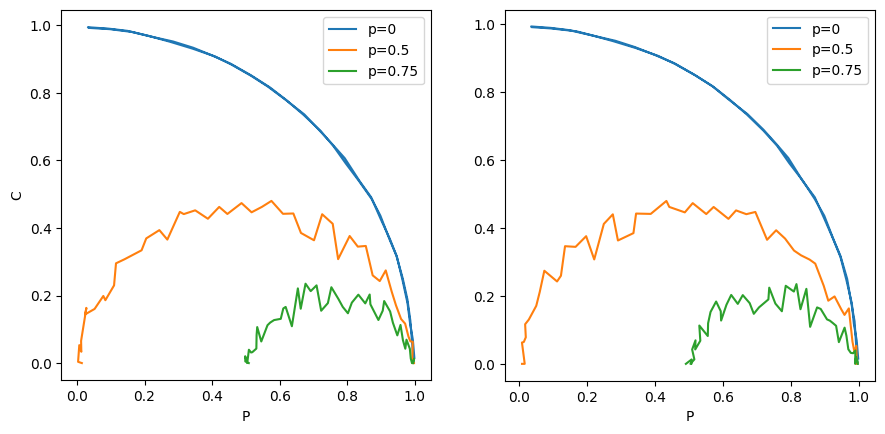
\includegraphics[width=300pt]{img/c_v_p_q2_v0.png}
			\captionof{figure}{Concurrence and polarization measured for 50 values of $\theta$ ranging from $0$ to $\pi$, and 3 values of $p$ shown on the graphs. The first graph shows the relationship for $P_0$ and the second one for $P_1$.}
			\label{c_v_p_q2}
		\end{center}
	
	\section{Two qubits ADC purification}
		We may reduce the quantum circuit to just 3 qubits if we consider the purification of the final state. First, we must consider that initial state
		$$
			|\psi_i\rangle=\cos(\theta)|01\rangle + \sin(\theta)|10\rangle
		$$
		will evolve to
		$$
		\rho_{01}=\mathcal{E}\left(\rho_{01}^{(0)}\right)=\sum_{\mu=0}^1 \sum_{v=0}^1 M_\mu^0 \otimes M_v^1\left(\rho_{01}^{(0)}\right) M_\mu^{0^{\dagger}} \otimes M_v^{1^{\dagger}},
		$$
		where $\rho_{01}^{(0)} = |\psi_i\rangle\langle\psi_i|$ and
		$$
		M_0=\left(\begin{array}{cc}
		1 & 0 \\
		0 & \sqrt{1-p}
		\end{array}\right), \quad M_1=\left(\begin{array}{cc}
		0 & \sqrt{p} \\
		0 & 0
		\end{array}\right)
		$$
		We are left with a final state
		$$
		\rho_{01}=\left(\begin{array}{cccc}
		p & 0 & 0 & 0 \\
		0 & (1-p) \cos ^2 \theta & (1-p) \cos \theta \sin \theta & 0 \\
		0 & (1-p) \cos \theta \sin \theta & (1-p) \sin ^2 \theta & 0 \\
		0 & 0 & 0 & 0
		\end{array}\right)
		$$
		Now to purify this state \cite{nielsen_quantum_2010} we must first express our state as
		$$
		\rho^A=\sum_i p_i\left|i^A\right\rangle\left\langle i^A\right|
		$$
		where each $|i^A\rangle$ forms an orthonormal basis. Then our pure state will be
		$$
		|A R\rangle \equiv \sum_i \sqrt{p_i}\left|i^A\right\rangle\left|i^R\right\rangle
		$$
		where $|i^A\rangle$ also forms an orthonormal basis belonging to system $R$.

		Therefore we may express our state of interest as
		$$
		\rho=p|00\rangle\langle 00|+(1-p)| \psi_i\rangle\langle\psi_i|
		$$
		and its pure state will be
		$$
		|\phi\rangle=\sqrt{p}|000\rangle+\sqrt{1-p}(\cos \theta|011\rangle+\sin \theta|101\rangle)
		$$
		where the last qubit belongs to the environment. If we consider that $\cos\varphi=\sqrt{p}$ and $\sin\varphi=\sqrt{1-p}$ we find a circuit that produces the state $|\phi\rangle$.

		\begin{center}
			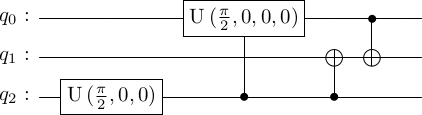
\includegraphics[width=200pt]{img/adc_2q_v1.png}
			\captionof{figure}{ADC for two qubits using 1 ancilla.}
			\label{adc_2q_v1}
		\end{center}

		Likewise we have used only the first parameter of U gate to set the values of $\varphi$ and $\theta$. Running this circuit on Qiskit quantum computer simulator we observe the same effect on the final states for different values of $p$.

		\begin{center}
			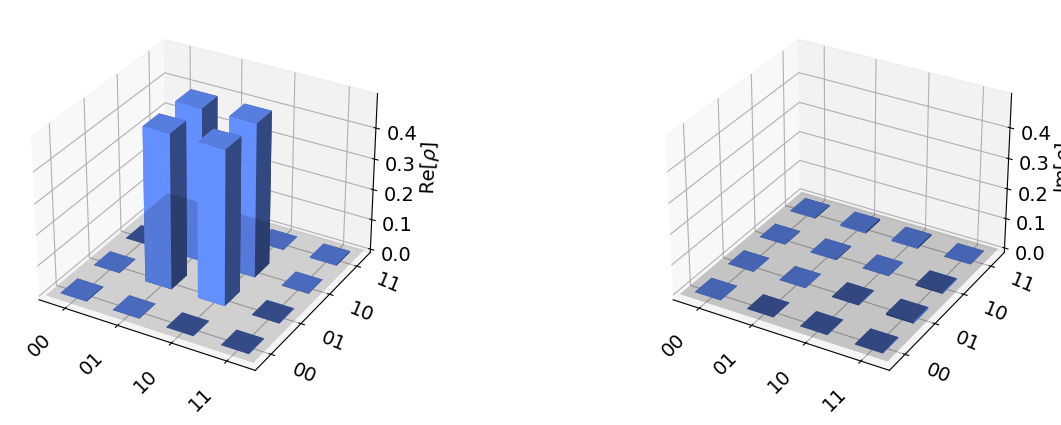
\includegraphics[width=300pt]{img/dm_p0_v1.png}
			\captionof{figure}{Final state for $p=0$.}
			\label{dm_p0}
		\end{center}

		\begin{center}
			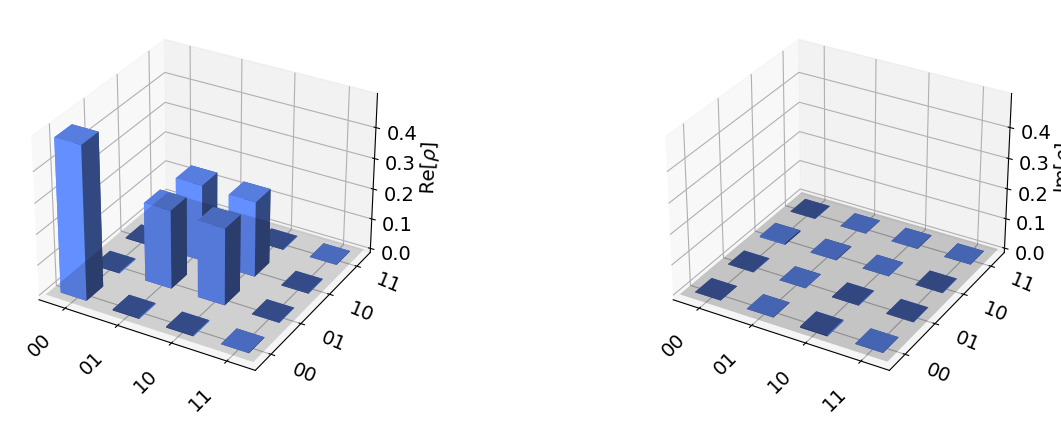
\includegraphics[width=300pt]{img/dm_p0.5_v1.png}
			\captionof{figure}{Final state for $p=0.5$.}
			\label{dm_p0.5}
		\end{center}

		\begin{center}
			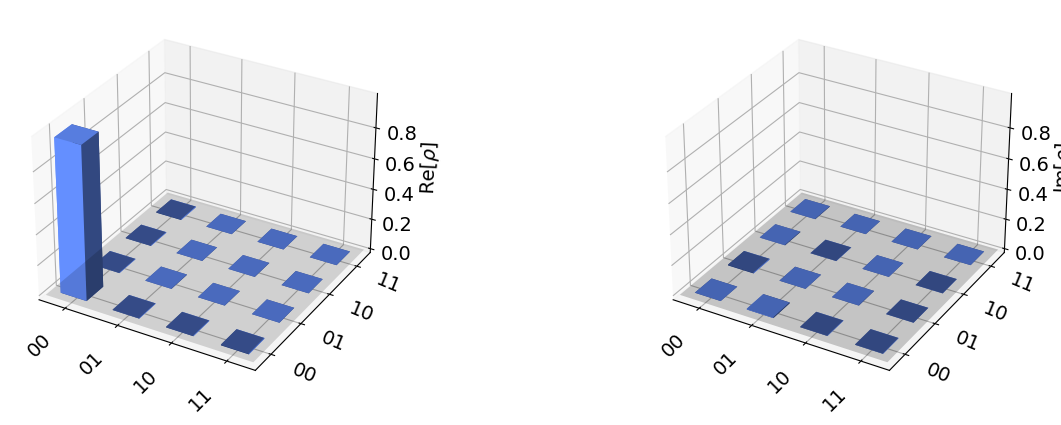
\includegraphics[width=300pt]{img/dm_p1_v1.png}
			\captionof{figure}{Final state for $p=1$.}
			\label{dm_p1}
		\end{center}

		We also see that the equations on \ref{cp_relation} hold.
		\begin{center}
			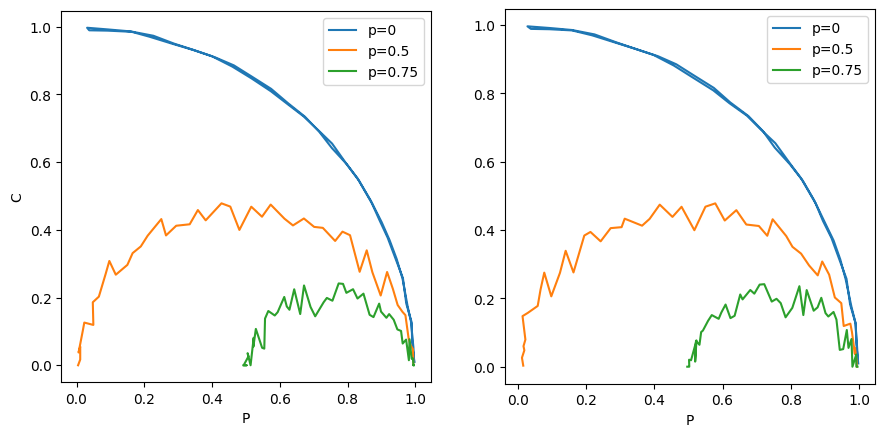
\includegraphics[width=300pt]{img/c_v_p_q2_v1.png}
			\captionof{figure}{Concurrence and polarization measured for 50 values of $\theta$ ranging from $0$ to $\pi$, and 3 values of $p$ shown on the graphs. The first graph shows the relationship for $P_0$ and the second one for $P_1$.}
			\label{c_v_p_q2}
		\end{center}
	\bibliography{citations}
	\bibliographystyle{ieeetr}
\end{document}